% Illustration of skip connection in a residual block. Inspired by the ResNet paper.
% https://arxiv.org/abs/1512.03385

\documentclass[tikz]{standalone}

\usetikzlibrary{positioning, calc, decorations.pathreplacing}

\begin{document}
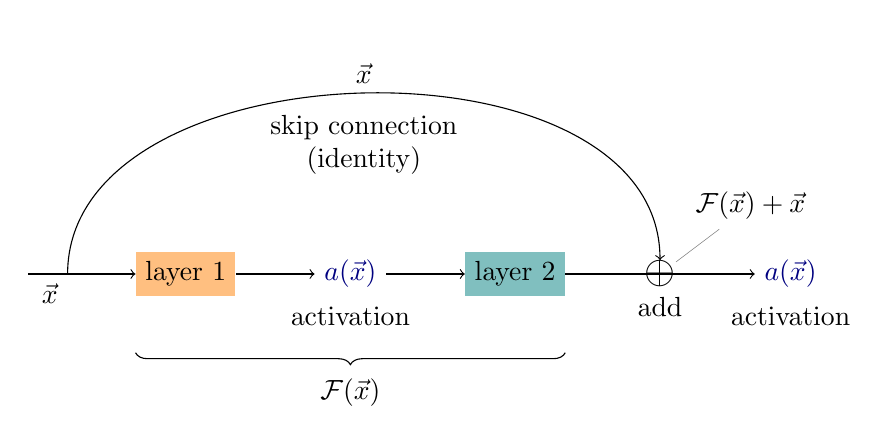
\begin{tikzpicture}

  \node[fill=orange!50] (l1) {layer 1};
  \node[blue!50!black, right=of l1, label={below:activation}] (act1) {$a(\vec x)$};
  \node[fill=teal!50, right=of act1] (l2) {layer 2};
  \node[right=of l2, font=\Large, label={below:add}, inner sep=0, pin={60:$\mathcal F(\vec x) + \vec x$}] (add) {$\oplus$};
  \node[blue!50!black, right=of add, label={below:activation}] (act2) {$a(\vec x)$};

  \draw[->] (l1) -- (act1);
  \draw[->] (act1) -- (l2);
  \draw[<-] (l1) -- ++(-2,0) node[below, pos=0.8] {$\vec x$};
  \draw[->] (l2) -- (act2) node[above, pos=0.8] {};
  \draw[->] ($(l1)-(1.5,0)$) to[out=90, in=90] node[below=1ex, midway, align=center] {skip connection\\(identity)} node[above, midway] {$\vec x$} (add);
  \draw[decorate, decoration={brace, amplitude=1ex, raise=1cm}] (l2.east) -- node[midway, below=1.2cm] {$\mathcal F(\vec x)$} (l1.west);

\end{tikzpicture}
\end{document}